\documentclass[a4 paper]{article}
% Set target color model to RGB
\usepackage[inner=2.0cm,outer=2.0cm,top=2.5cm,bottom=2.5cm]{geometry}
\usepackage{graphicx}
\usepackage[table,xcdraw]{xcolor}
\usepackage{tikz}
\usepackage{colortbl}
% \usepackage[final]{graphicx}
\usetikzlibrary{positioning, shadows, arrows, trees, shapes, fit}
% \usepackage[spanish]{babel}
\usepackage[spanish,es-tabla]{babel}
\usepackage{setspace}

\usepackage{multirow}
\usepackage[table,xcdraw]{xcolor}
% \doublespacing
\onehalfspace
% \singlespace
% \spacing{1.5}

% \usepackage[rgb]{xcolor}
\usepackage{verbatim}
% \usepackage[demo]{graphicx}
% \usepackage{caption}
\usepackage{subcaption}
\usepackage{amsgen,amsmath,amstext,amsbsy,amsopn,tikz,amssymb,tkz-linknodes}
\usepackage{siunitx}
\usepackage{fancyhdr}
\usepackage[colorlinks=true, urlcolor=blue,  linkcolor=blue, citecolor=blue]{hyperref}
\usepackage[colorinlistoftodos]{todonotes}
\usepackage{rotating}
% \usetikzlibrary{through,backgrounds}
\hypersetup{%
pdfauthor={Ashudeep Singh},%
pdftitle={Homework},%
pdfkeywords={Tikz,latex,bootstrap,uncertaintes},%
pdfcreator={PDFLaTeX},%
pdfproducer={PDFLaTeX},%
}

%\usetikzlibrary{shadows}
% \usepackage[francais]{babel}
% \usepackage[spanish]{babel}
\usepackage[utf8]{inputenc}
\usepackage[T1]{fontenc}
\usepackage{pdfpages}
\usepackage{boldline,multirow,tabularx,colortbl,diagbox,makecell,fancybox}

\usepackage{color}
\usepackage{fancyvrb}

\usepackage{subcaption}

\usepackage{amsfonts,amssymb,amsmath,mathrsfs,array,stmaryrd}
\usepackage{pgf,tikz,xcolor}
\usetikzlibrary{calc,positioning,shapes.geometric,shapes.symbols,shapes.misc, fit, shapes, arrows, arrows.meta}
\usepackage{setspace}
\usepackage{fancyhdr}
\usepackage{indentfirst}
\usepackage{hyperref}
\usepackage[nottoc]{tocbibind}
\usepackage{float}

\usetikzlibrary{arrows}
\usepackage{graphicx}
% \usepackage{subfig}
% \usepackage{amsmath} % assumes amsmath package installed
% \usepackage{amssymb}  % assumes amsmath package installed
% \usepackage{xspace}
% \usepackage{ifthen}
% \usepackage{xcolor}

\usepackage{enumerate}
\usepackage[pstricks1-10]{vaucanson-g}


\usepackage{listings}
\lstset{language=Python}%, basicstyle=\ttfamily}
\usepackage{amsmath}

\newcommand{\ra}[1]{\renewcommand{\arraystretch}{#1}}

\newtheorem{thm}{Theorem}[section]
\newtheorem{prop}[thm]{Proposition}
\newtheorem{lem}[thm]{Lemma}
\newtheorem{cor}[thm]{Corollary}
\newtheorem{defn}[thm]{Definition}
\newtheorem{rem}[thm]{Remark}
\numberwithin{equation}{section}

\newcommand{\homework}[6]{
   \pagestyle{myheadings}
   \thispagestyle{plain}
   \newpage
   \setcounter{page}{1}
   \noindent
   \begin{center}
   \framebox{
      \vbox{\vspace{2mm}
    \hbox to 6.28in { {\bf Cátedra: Aprendizaje Profundo y Redes Neuronales Artificiales \hfill {\small (#2)}} }
       \vspace{6mm}
       \hbox to 6.28in { {\Large \hfill #1  \hfill} }
       \vspace{6mm}
       \hbox to 6.28in { {\it Docentes: {\rm #3} \hfill Alumnos: {\rm #5}, {\rm #6}} }
       %\hbox to 6.28in { {\it TA: #4  \hfill #6}}
      \vspace{2mm}}
   }
   \end{center}
   \markboth{#5 -- #1}{#5 -- #1}
   \vspace*{4mm}
}

\newcommand{\problem}[2]{~\\\fbox{\textbf{Problem #1}}\hfill (#2 points)\newline\newline}
\newcommand{\subproblem}[1]{~\newline\textbf{(#1)}}
\newcommand{\D}{\mathcal{D}}
\newcommand{\Hy}{\mathcal{H}}
\newcommand{\VS}{\textrm{VS}}
\newcommand{\solution}{~\newline\textbf{\textit{(Solution)}} }

\newcommand{\bbF}{\mathbb{F}}
\newcommand{\bbX}{\mathbb{X}}
\newcommand{\bI}{\mathbf{I}}
\newcommand{\bX}{\mathbf{X}}
\newcommand{\bY}{\mathbf{Y}}
\newcommand{\bepsilon}{\boldsymbol{\epsilon}}
\newcommand{\balpha}{\boldsymbol{\alpha}}
\newcommand{\bbeta}{\boldsymbol{\beta}}
\newcommand{\0}{\mathbf{0}}


\newcommand{\comments}[1]{}

\newboolean{showcomments}
\setboolean{showcomments}{true} % comment this line to deactivate comments
\ifthenelse{\boolean{showcomments}}{
	\newcommand{\nbc}[3]{
		{\colorbox{#3}{\bfseries\sffamily\scriptsize\textcolor{white}{#1}}}
		{\textcolor{#3}{\sf\small$\langle$\textit{#2}$\rangle$}}}
}{
	\newcommand{\nbc}[3]{}
	\newcommand{\version}{}
}


\newcommand{\tc}[1]{\nbc{TC}{#1}{red}} 
\newcommand{\tl}[1]{\nbc{TL}{#1}{blue}}


\begin{document}
\newcommand{\addstudent}[3]{\small{#1} & \small{#2} & \small{\href{mailto:#3}{#3}}\\}
\newcommand{\addtutor}[2]{#1 & #2\\}
%==[DO NOT CHANGE ANYTHING BEFORE THIS LINE]====================

% Your PIR project title here
\def\projecttitle{
    % Template State of the Art for a great PIR Project
    Trabajo Práctico Nº 2:   Introducción a las Redes Neuronales
}
\def\catedra{Aprendizaje Profundo y Redes Neuronales Artificiales}

% Your keywords here
\def\varkeywords{
    Keyword 1; Keyword 2; Keyword 3; Keyword 4; Keyword 5 
}

% Your names here
\def\students{
    \addstudent{Tomás}{LIENDRO}{tomas.liendro@ib.edu.ar}
    % \addstudent{Sol M.}{MALDONADO BETANZO}{solmabet@hotmail.com}
}

% Your tutors here
\def\tutors{
    \addtutor{Ariel}{CURIALE}
    \addtutor{Germán}{MATO}
    \addtutor{Lucca}{DELLAZOPPA}
}

\newcommand\tab[1][0.6cm]{\hspace*{#1}} %Create and define tab


%Chapter No Numbering but appears in TOC
\newcommand{\chapternn}[1]{\chapter*{#1}\addcontentsline{toc}{chapter}{#1}}
\newcommand{\sectionnn}[1]{\section*{#1}\addcontentsline{toc}{section}{#1}}
\newcommand{\subsectionnn}[1]{\subsection*{#1}\addcontentsline{toc}{subsection}{#1}}
\newcommand{\subsubsectionnn}[1]{\subsubsection*{#1}\addcontentsline{toc}{subsubsection}{#1}}

\newcolumntype{L}[1]{>{\raggedright\arraybackslash\hspace{0pt}}p{#1}}
\newcolumntype{R}[1]{>{\raggedleft\arraybackslash\hspace{0pt}}p{#1}}
\newcolumntype{C}[1]{>{\centering\arraybackslash\hspace{0pt}}p{#1}}

\renewcommand\thesection{\arabic{section}}
\renewcommand\thesubsection{\thesection.\arabic{subsection}}


% \RequirePackage{fancyhdr}
\pagestyle{fancy}

%------- Do not append new commands after :

\hypersetup{	
    colorlinks  = false, % colorise les liens
    linkbordercolor = {1 1 1},
    breaklinks  = true, % permet le retour à la ligne dans les liens trop longs
    urlcolor    = blue, % couleur des hyperliens 
    linkcolor   = black,	% couleur des liens internes 
    citecolor   = black,	% couleur des références 
    pdftitle    = {Security assessment of connected objects in the Internet of Things : State of the art}, % informations apparaissant dans 
    pdfauthor   = {}, % les informations du document 
    pdfsubject  = {}	% sous Acrobat. 
}

\title{\vspace{3.5cm}  \\ \vspace{0.25cm} \LARGE{\textbf{\projecttitle}} \\ \vspace{0.25cm}
\vspace{0.25cm} \LARGE{{\catedra}}}
% \vspace{7.25cm}
\author{}
\date{\today}

% \RequirePackage{fancyhdr}
\pagestyle{fancy}
\renewcommand{\headrule}{}
\lhead{}
\chead{}
\rhead{}
\lfoot{\projecttitle}
\cfoot{}
\rfoot{\thepage}

\AtBeginDocument{\pagenumbering{gobble}
\thispagestyle{empty}

\pagenumbering{gobble}
\maketitle
\vspace{0.5cm}
\vspace{1cm}

\hrule
\vspace{1cm}

\noindent\begin{tikzpicture}[remember picture, overlay, shift={(current page.south west)}]
    %Images
    \node[anchor=north west] at (2,27.7) {
\includegraphics[height=3cm, keepaspectratio]{cover/meta/cnea.png}};
    % \node[anchor=north west] at (2,26.25) {Département de Génie Électrique \& Informatique};
    \node[anchor=north] at (10.5,27.7) {
\includegraphics[height=3cm]{cover/meta/ib.png}};
    %\node[anchor=north east] at (21-2,27.7) {\includegraphics[height=1.225cm, keepaspectratio]{cover/meta/laas.jpg}};
    \node[anchor=north east] at (21-2,27.7) {
\includegraphics[height=3cm, keepaspectratio]{cover/meta/uncu2.png}};
\end{tikzpicture}

\vspace{1cm}

\begin{center}
    \textbf{Alumnos :}
    \vspace{0.25cm}
    
    \begin{tabular}{lll}
        \students
    \end{tabular}
\end{center}
\vspace{0.5cm}

\begin{center}
    \textbf{Docentes :}
    \vspace{0.25cm}
    
    \begin{tabular}{lll}
        \tutors
    \end{tabular}
\end{center}\vspace{0.2cm}

% \begin{center}
%     \textbf{Keywords:}
%     \varkeywords
% \end{center}
% \vspace{0.5cm}


\begin{center}
\vfill
{\Large {San Carlos de Bariloche, Argentina}}
\end{center}

\newpage

\pagestyle{fancy}
\lhead{}
\chead{}
\rhead{}
\lfoot{\projecttitle}
\cfoot{}
\rfoot{}
\doublespacing
\tableofcontents
\singlespacing
\newpage

\pagenumbering{arabic}
\pagestyle{fancy}
\lhead{}
\chead{}
\rhead{}
\lfoot{\projecttitle}
\cfoot{}
\rfoot{\thepage}}

\AtEndDocument{\input{cover/cover_out.tex}}


% % \begin{center}
%     \Large{\textbf{Resumen :}}
% \end{center}
\section{Resumen}

Este trabajo consiste en la integración de los conocimientos adquiridos en la materia para comandar un manipulador robótico.
Haciendo uso de un entorno de simulación implementado en \textit{Python} con la librería \textit{Panda3D} se pudo verificar el comportamiento del robot frente a distintos escenarios en los cuales debe: 1) identificar una pieza cargada en una base de datos mediante algún método de procesamiento de imágenes, 2) determinar las matrices de transformación homogéneas que permitirán al robot tomar la pieza, 3) depositar la pieza en una posición específica predeterminada moviéndose en un entorno libre de obstáculos, 4) integrar el algoritmo de \textit{motion planning} de Dijkstra para depositar la pieza en una posición específica predeterminada moviéndose en un entorno con obstáculos.
Gran parte de este trabajo se basó en informes previos realizados en los cuales se abordaron los temas de cinemática directa y cinemática inversa.

% En el presente trabajo se utiliza el lenguaje de programación \textit{Python 3} en conjunto con el paquete \textit{Panda3D} para poder simular al robot RM501. Con el mismo, se cumplen distintas misiones, en donde le objetivo principal es reconocer distintas piezas, buscarlas y dejarlas en el lugar indicado. También, se plantean distintos escenarios con obstáculos que el robot debe esquivar, planificando su trayectoria con el algoritmo de Dijkstra de \textit{motion planning}.
% % \begin{center}
%     \Large{\textbf{Resumen :}}
% \end{center}
\section{Resumen}

Este trabajo consiste en la integración de los conocimientos adquiridos en la materia para comandar un manipulador robótico.
Haciendo uso de un entorno de simulación implementado en \textit{Python} con la librería \textit{Panda3D} se pudo verificar el comportamiento del robot frente a distintos escenarios en los cuales debe: 1) identificar una pieza cargada en una base de datos mediante algún método de procesamiento de imágenes, 2) determinar las matrices de transformación homogéneas que permitirán al robot tomar la pieza, 3) depositar la pieza en una posición específica predeterminada moviéndose en un entorno libre de obstáculos, 4) integrar el algoritmo de \textit{motion planning} de Dijkstra para depositar la pieza en una posición específica predeterminada moviéndose en un entorno con obstáculos.
Gran parte de este trabajo se basó en informes previos realizados en los cuales se abordaron los temas de cinemática directa y cinemática inversa.

% En el presente trabajo se utiliza el lenguaje de programación \textit{Python 3} en conjunto con el paquete \textit{Panda3D} para poder simular al robot RM501. Con el mismo, se cumplen distintas misiones, en donde le objetivo principal es reconocer distintas piezas, buscarlas y dejarlas en el lugar indicado. También, se plantean distintos escenarios con obstáculos que el robot debe esquivar, planificando su trayectoria con el algoritmo de Dijkstra de \textit{motion planning}.
% \input{content/abstract}



\section{Ejercicio 1}

En este trabajo se abordaron los conceptos de \textit{Computational Graphs} y \textit{Back Propagation} para entrenar una red neuronal densa.
Un \textbf{grafo computacional} es una manera de representar una función matemática en el lenguaje de la teoría de grafos. En el grafo, cada nodo representa un valor de una variable o una función que combina valores. Los valores que ingresan o salen de los nodos se denominan \textbf{Tensores}.

Utilizando el concepto de \textbf{grafos computacionales} se busca implementar las funciones \textbf{Sigmoide}, \textbf{Tanh}, \textbf{ELU} y \textbf{Leaky Relu}, tomando como entrada:
$x=[2.8, -1.8]$, $W=[1.45, -0.35]$, $b=-4$. En los siguientes grafos, los valores en color negro indican los resultados del proceso hacia adelante (\textit{forward}) mientras que en rojo se colocan los resultados del \textit{Backpropagation} recordando que el valor del gradiente a la salida del grafo es 1.

\subsection{Sigmoide}

\begin{equation}
    f(x)=\frac{1}{1+e^{-x}};\ \ f'(x)=\sigma(x)(1-\sigma(x))
\end{equation}
\vspace{1cm}
\hspace{1.5cm}
% first of all, we define our grid
\begin{VCPicture}{(0,-3)(6,3)}

% and then we create the states
\ChgEdgeLabelScale{0.5}
\ChgEdgeLabelSep{.5}
\LargeState
\VSState{(-1.5,1.5)}{S1}
\VSState{(-1.5,0)}{S2}
\VSState{(-1.5,-1.5)}{S3}
\VSState{(-1.5,-3)}{S4}
\VSState{(-1.5,-4.5)}{S5}

\State[w_0]{(0,1.5)}{STATEA}
\State[x_0]{(0,0)}{STATEB}
\State[w_1]{(0,-1.5)}{STATEC}
\State[x_1]{(0,-3)}{STATED}
\State[b]{(2,-4.5)}{STATEE}

\State[\times]{(2,0.75)}{STATEF}
\State[\times]{(2,-2.25)}{STATEG}

\State[+]{(4.5,-.75)}{STATEH}


\StateVar[\times(-1)]{(7,-.75)}{STATEI}

\State[\exp]{(9.5,-.75)}{STATEJ}
\State[+1]{(11.5,-.75)}{STATEK}
\State[1/x]{(13.5,-.75)}{STATEL}
\VSState{(15.5,-.75)}{ENDSTATE}
% now, transition time

% straight lines
\EdgeR{S1}{STATEA}{1.45}
\EdgeR{S2}{STATEB}{2.8}
\EdgeR{S3}{STATEC}{-0.35}
\EdgeR{S4}{STATED}{-1.8}
\EdgeR{S5}{STATEE}{-4}

\LArcR{STATEA}{STATEF}{}
\LArcL{STATEB}{STATEF}{}
\LArcR{STATEC}{STATEG}{}
\LArcL{STATED}{STATEG}{}

\ArcR{STATEF}{STATEH}{4.060}
\ArcR{STATEG}{STATEH}{0.630}
\LArcR{STATEE}{STATEH}{}

\LArcL{STATEH}{STATEI}{0.690}
\LArcL{STATEI}{STATEJ}{-0.690}
\LArcL{STATEJ}{STATEK}{1.994}
\LArcL{STATEK}{STATEL}{2.994}

\EdgeR{STATEL}{ENDSTATE}{0.334}

\ChgEdgeLineColor{red}
\ChgEdgeLineStyle{dashed}
\ChgEdgeLabelColor{red}

\LArcL{STATEL}{STATEK}{-0.112}
\LArcL{STATEK}{STATEJ}{-0.112}
\LArcL{STATEJ}{STATEI}{-0.056}
\LArcL{STATEI}{STATEH}{0.056}

\ArcR{STATEH}{STATEF}{0.056}
\ArcR{STATEH}{STATEG}{0.056}
\ArcL{STATEH}{STATEE}{0.056}

\LArcR{STATEF}{STATEA}{0.157}
\LArcL{STATEF}{STATEB}{0.081}
\LArcR{STATEG}{STATEC}{-0.101}
\LArcL{STATEG}{STATED}{-0.020}


% loops
% \LoopN{STATEA}{0.1}
% \LoopW{STATEB}{0.4}
% \LoopE{STATED}{0.6}

\end{VCPicture}
\newline

\begin{figure}[H]
    \centering
    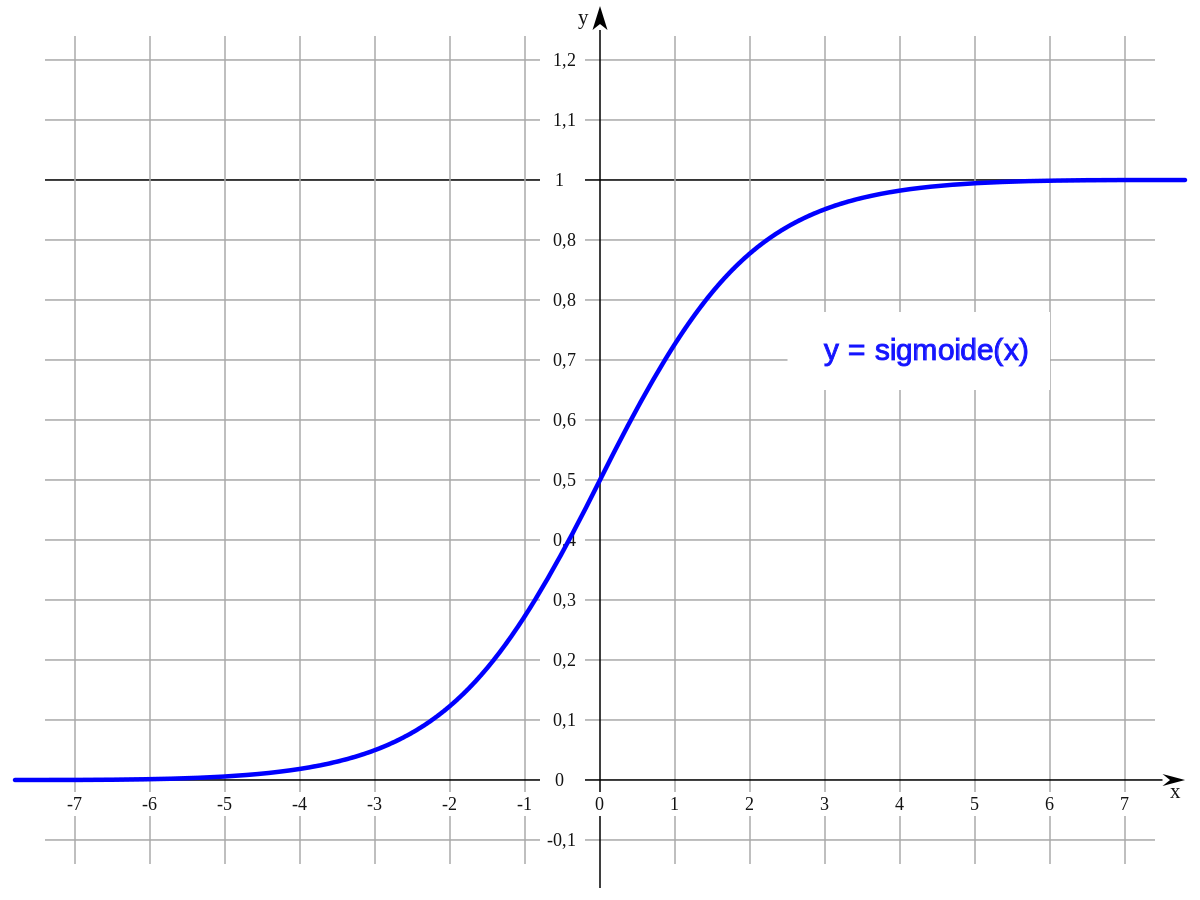
\includegraphics[height=2in]{image/sigmoide}
    \caption{Función Sigmoide ($\sigma(x))$}
    \label{fig:my_label}
\end{figure}


\subsection{Tanh}

\begin{equation}
    f(x)=tanh(x)=\frac{e^{-x}-1}{e^{-x}+1}; \ \ f'(x)=1-tanh^2(x)
\end{equation}
\vspace{1cm}
\hspace{1.5cm}
% first of all, we define our grid
\begin{VCPicture}{(0,-3)(6,3)}

% and then we create the states
\ChgEdgeLabelScale{0.5}
% \ChgEdgeLabelSep{}
\LargeState
\VSState{(-1.5,1.5)}{S1}
\VSState{(-1.5,0)}{S2}
\VSState{(-1.5,-1.5)}{S3}
\VSState{(-1.5,-3)}{S4}
\VSState{(-1.5,-4.5)}{S5}

\State[w_0]{(0,1.5)}{STATEA}
\State[x_0]{(0,0)}{STATEB}
\State[w_1]{(0,-1.5)}{STATEC}
\State[x_1]{(0,-3)}{STATED}
\State[b]{(2,-4.5)}{STATEE}

\State[\times]{(2,0.75)}{STATEF}
\State[\times]{(2,-2.25)}{STATEG}

\State[+]{(4.5,-.75)}{STATEH}


\StateVar[\times(2)]{(6.5,-.75)}{STATEI}

\State[\exp]{(9,-.75)}{STATEJ}

\State[-1]{(11,1)}{STATEK}
\State[+1]{(11,-2.5)}{STATEL}

\State[\frac{a}{b}]{(13,-.75)}{STATEM}

\VSState{(15,-.75)}{ENDSTATE}
% now, transition time

% straight lines
\EdgeR{S1}{STATEA}{1.45}
\EdgeR{S2}{STATEB}{2.8}
\EdgeR{S3}{STATEC}{-0.35}
\EdgeR{S4}{STATED}{-1.8}
\EdgeR{S5}{STATEE}{-4}

\LArcR{STATEA}{STATEF}{}
\LArcL{STATEB}{STATEF}{}
\LArcR{STATEC}{STATEG}{}
\LArcL{STATED}{STATEG}{}

\ArcR{STATEF}{STATEH}{4.060}
\ArcR{STATEG}{STATEH}{0.630}
\LArcR{STATEE}{STATEH}{}

\LArcL{STATEH}{STATEI}{0.690}
\LArcL{STATEI}{STATEJ}{1.38}
% \ArcL{A}{B}{\IOL{2}{0}}
\LArcL{STATEJ}{STATEK}{3.975}
\LArcR{STATEJ}{STATEL}{3.975}

\LArcL{STATEK}{STATEM}{2.975}
\LArcR{STATEL}{STATEM}{4.975}

\EdgeR{STATEM}{ENDSTATE}{0.598}

\ChgEdgeLineColor{red}
\ChgEdgeLineStyle{dashed}
\ChgEdgeLabelColor{red}

\ArcR{STATEM}{STATEL}{-0.120}
\ArcL{STATEM}{STATEK}{0.201}

\ArcR{STATEL}{STATEJ}{-0.120}
\ArcL{STATEK}{STATEJ}{0.201}

\LArcL{STATEJ}{STATEI}{0.322}
\LArcL{STATEI}{STATEH}{0.644}

\ArcR{STATEH}{STATEF}{0.644}
\ArcR{STATEH}{STATEG}{0.644}
\ArcL{STATEH}{STATEE}{0.644}

\LArcR{STATEF}{STATEA}{1.803}
\LArcL{STATEF}{STATEB}{0.934}
\LArcR{STATEG}{STATEC}{-1.159}
\LArcL{STATEG}{STATED}{-0.225}



% loops
% \LoopN{STATEA}{0.1}
% \LoopW{STATEB}{0.4}
% \LoopE{STATED}{0.6}

\end{VCPicture}
\newline

\begin{figure}[H]
    \centering
    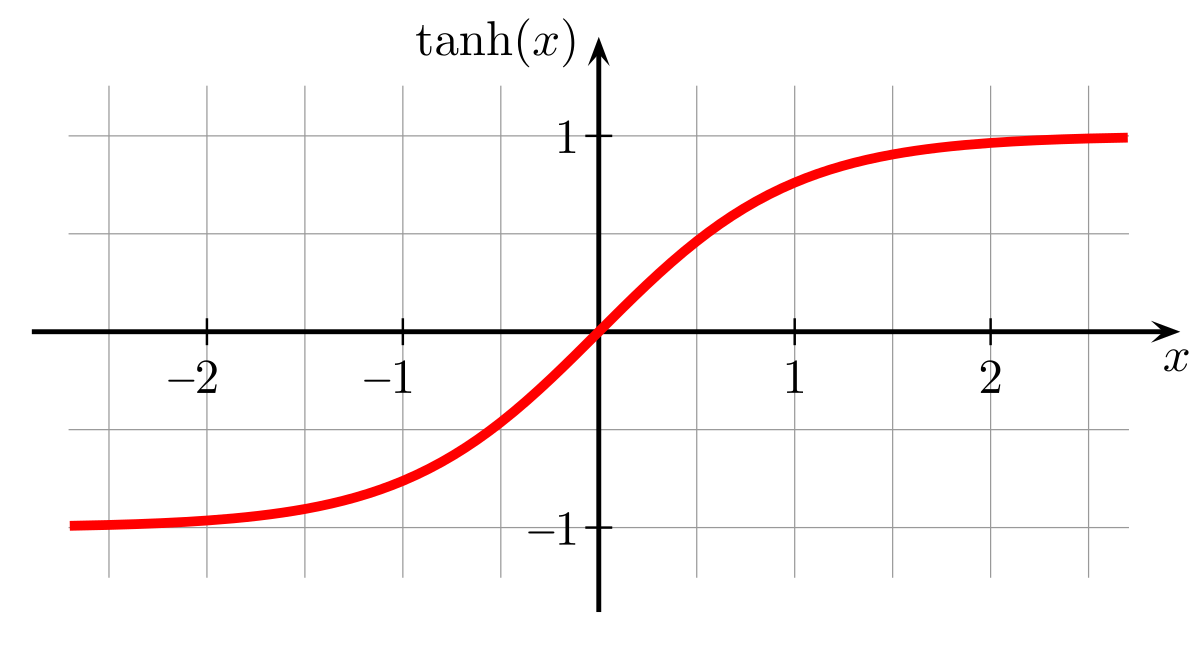
\includegraphics[height=2in]{image/tanh}
    \caption{Función Tangente Hiperbólica ($tanh(x)$)}
    \label{fig:my_label}
\end{figure}

\subsection{ELU}

\[   
f(a,b) = 
     \begin{cases}
        \text{x} & x \geq 0 \\
       \text{$\alpha (\exp(x)-1)$} & x < 0 \\
     \end{cases}
\]
\vspace{1cm}
\hspace{5.5cm}
% first of all, we define our grid
\begin{VCPicture}{(0,-3)(6,3)}

% and then we create the states
\ChgEdgeLabelScale{0.5}
\ChgEdgeLabelSep{.5}
\LargeState
\VSState{(-1.5,1.5)}{S1}
\VSState{(-1.5,0)}{S2}
\VSState{(-1.5,-1.5)}{S3}
\VSState{(-1.5,-3)}{S4}
\VSState{(-1.5,-4.5)}{S5}

\State[w_0]{(0,1.5)}{STATEA}
\State[x_0]{(0,0)}{STATEB}
\State[w_1]{(0,-1.5)}{STATEC}
\State[x_1]{(0,-3)}{STATED}
\State[b]{(2,-4.5)}{STATEE}

\State[\times]{(2,0.75)}{STATEF}
\State[\times]{(2,-2.25)}{STATEG}

\State[+]{(4.5,-.75)}{STATEH}


% \StateVar[\times(-1)]{(7,-.75)}{STATEI}

% \State[\exp]{(9.5,-.75)}{STATEJ}
% \State[+1]{(11.5,-.75)}{STATEK}
% \State[1/x]{(13.5,-.75)}{STATEL}
\VSState{(7,-.75)}{ENDSTATE}
% now, transition time

% straight lines
\EdgeR{S1}{STATEA}{1.45}
\EdgeR{S2}{STATEB}{2.8}
\EdgeR{S3}{STATEC}{-0.35}
\EdgeR{S4}{STATED}{-1.8}
\EdgeR{S5}{STATEE}{-4}

\LArcR{STATEA}{STATEF}{}
\LArcL{STATEB}{STATEF}{}
\LArcR{STATEC}{STATEG}{}
\LArcL{STATED}{STATEG}{}

\ArcR{STATEF}{STATEH}{4.060}
\ArcR{STATEG}{STATEH}{0.630}
\LArcR{STATEE}{STATEH}{}

% \LArcL{STATEH}{STATEI}{0.690}
% \LArcL{STATEI}{STATEJ}{-0.690}
% \LArcL{STATEJ}{STATEK}{1.994}
% \LArcL{STATEK}{STATEL}{2.994}

\EdgeR{STATEH}{ENDSTATE}{0.0.690}

\ChgEdgeLineColor{red}
\ChgEdgeLineStyle{dashed}
\ChgEdgeLabelColor{red}

% \LArcL{STATEL}{STATEK}{-0.112}
% \LArcL{STATEK}{STATEJ}{-0.112}
% \LArcL{STATEJ}{STATEI}{-0.056}
% \LArcL{STATEI}{STATEH}{0.056}

\ArcR{STATEH}{STATEF}{1}
\ArcR{STATEH}{STATEG}{1}
\ArcL{STATEH}{STATEE}{1}

\LArcR{STATEF}{STATEA}{2.8}
\LArcL{STATEF}{STATEB}{1.450}
\LArcR{STATEG}{STATEC}{-1.800}
\LArcL{STATEG}{STATED}{-0.350}


% loops
% \LoopN{STATEA}{0.1}
% \LoopW{STATEB}{0.4}
% \LoopE{STATED}{0.6}

\end{VCPicture}
\newline
\vspace{1cm}
\hspace{1.5cm}
% first of all, we define our grid
\begin{VCPicture}{(0,-3)(6,3)}

% and then we create the states
\ChgEdgeLabelScale{0.5}
\ChgEdgeLabelSep{.5}
\LargeState
\VSState{(-1.5,1.5)}{S1}
\VSState{(-1.5,0)}{S2}
\VSState{(-1.5,-1.5)}{S3}
\VSState{(-1.5,-3)}{S4}
\VSState{(-1.5,-4.5)}{S5}

\State[w_0]{(0,1.5)}{STATEA}
\State[x_0]{(0,0)}{STATEB}
\State[w_1]{(0,-1.5)}{STATEC}
\State[x_1]{(0,-3)}{STATED}
\State[b]{(2,-4.5)}{STATEE}

\State[\times]{(2,0.75)}{STATEF}
\State[\times]{(2,-2.25)}{STATEG}

\State[+]{(4.5,-.75)}{STATEH}


\State[\exp]{(7,-.75)}{STATEI}
\State[-1]{(9.5,-.75)}{STATEJ}
\StateVar[\times\alpha]{(12,-.75)}{STATEK}
\VSState{(14.5,-.75)}{ENDSTATE}
% now, transition time

% straight lines
\EdgeR{S1}{STATEA}{1.45}
\EdgeR{S2}{STATEB}{2.8}
\EdgeR{S3}{STATEC}{-0.35}
\EdgeR{S4}{STATED}{-1.8}
\EdgeR{S5}{STATEE}{-4}

\LArcR{STATEA}{STATEF}{}
\LArcL{STATEB}{STATEF}{}
\LArcR{STATEC}{STATEG}{}
\LArcL{STATED}{STATEG}{}

\ArcR{STATEF}{STATEH}{4.060}
\ArcR{STATEG}{STATEH}{0.630}
\LArcR{STATEE}{STATEH}{}

\LArcL{STATEH}{STATEI}{0.690}

\LArcL{STATEI}{STATEJ}{1.994}
\LArcL{STATEJ}{STATEK}{0.994}
\EdgeR{STATEK}{ENDSTATE}{\alpha 0.994}

% \EdgeR{STATEK}{ENDSTATE}{\alpha 0.994}

\ChgEdgeLineColor{red}
\ChgEdgeLineStyle{dashed}
\ChgEdgeLabelColor{red}

% \LArcL{STATEL}{STATEK}{-0.112}
\LArcL{STATEK}{STATEJ}{\alpha}
\LArcL{STATEJ}{STATEI}{\alpha}
\LArcL{STATEI}{STATEH}{\alpha 1.994}

\ArcR{STATEH}{STATEF}{\alpha 1.994}
\ArcR{STATEH}{STATEG}{\alpha 1.994}
\ArcL{STATEH}{STATEE}{\alpha 1.994}

\LArcR{STATEF}{STATEA}{\alpha 5.583}
\LArcL{STATEF}{STATEB}{\alpha 2.891}
\LArcR{STATEG}{STATEC}{-\alpha 3.589}
\LArcL{STATEG}{STATED}{-\alpha 0.698}


% loops
% \LoopN{STATEA}{0.1}
% \LoopW{STATEB}{0.4}
% \LoopE{STATED}{0.6}

\end{VCPicture}
\newline
\newline

\begin{figure}[H]
    \centering
    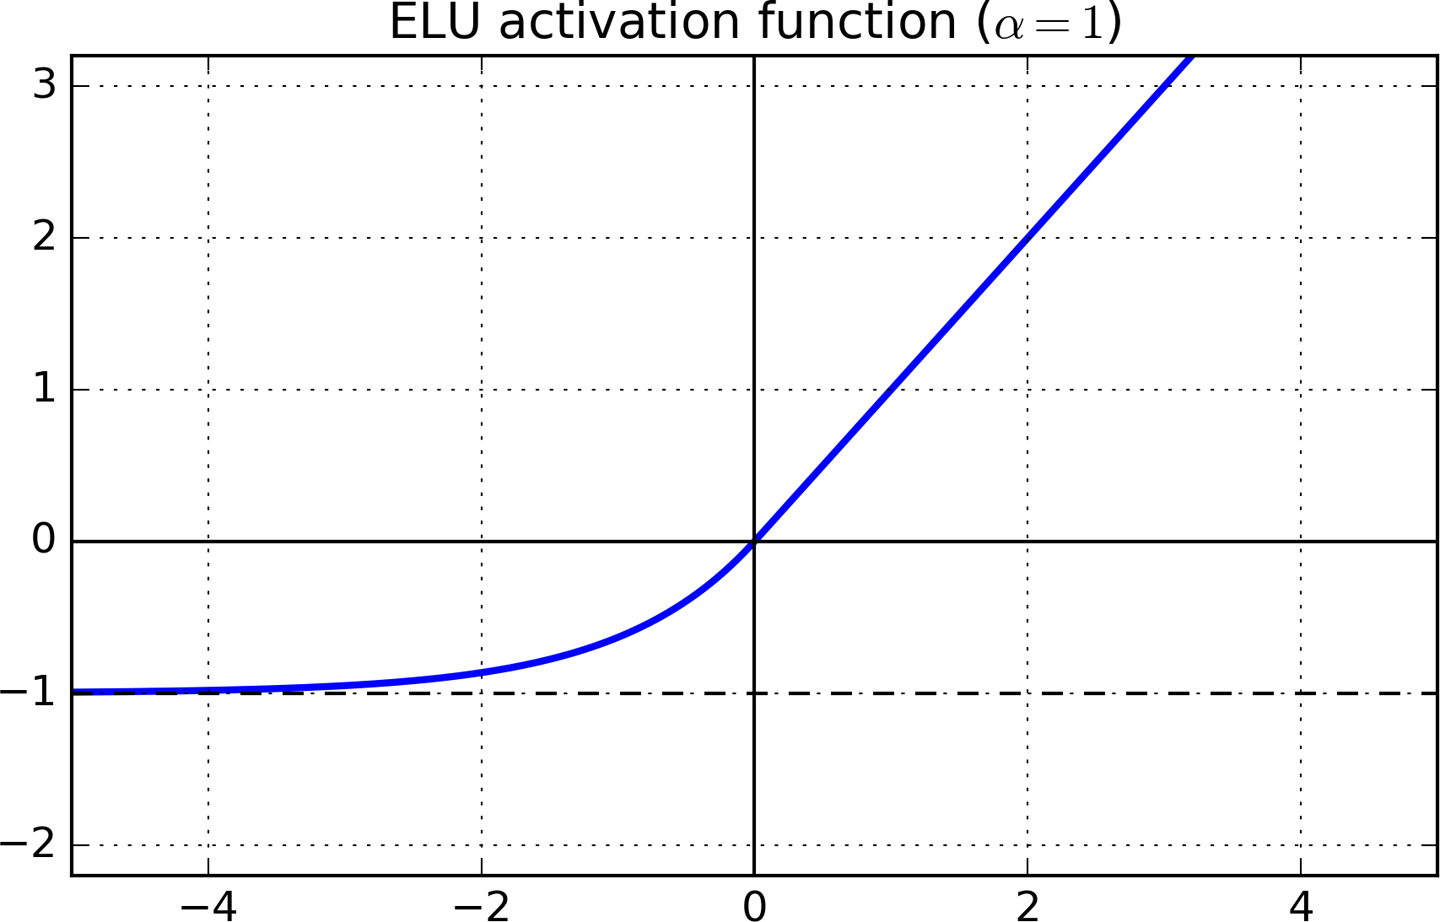
\includegraphics[height=2in]{image/ELU}
    \caption{Función de activación ELU}
    \label{fig:my_label}
\end{figure}



\subsection{Leaky Relu}

\begin{equation}
    f(x)=LeakyRelu(x)=max(0.1x, x)
\end{equation}
\vspace{1cm}
\hspace{3.5cm}
% first of all, we define our grid
\begin{VCPicture}{(0,-3)(6,3)}

% and then we create the states
\ChgEdgeLabelScale{0.5}
% \ChgEdgeLabelSep{}
\LargeState
\VSState{(-1.5,1.5)}{S1}
\VSState{(-1.5,0)}{S2}
\VSState{(-1.5,-1.5)}{S3}
\VSState{(-1.5,-3)}{S4}
\VSState{(-1.5,-4.5)}{S5}

\State[w_0]{(0,1.5)}{STATEA}
\State[x_0]{(0,0)}{STATEB}
\State[w_1]{(0,-1.5)}{STATEC}
\State[x_1]{(0,-3)}{STATED}
\State[b]{(2,-4.5)}{STATEE}

\State[\times]{(2,0.75)}{STATEF}
\State[\times]{(2,-2.25)}{STATEG}

\State[+]{(4.5,-.75)}{STATEH}


\StateVar[\times(0.1)]{(6.5,1)}{STATEI}
\StateVar[\times 1]{(6.5,-2.5)}{STATEJ}
% \State[\exp]{(9,-.75)}{STATEJ}

\StateVar[MAX]{(9,-.75)}{STATEK}
% \State[+1]{(11,-2.5)}{STATEL}

% \State[\frac{a}{b}]{(13,-.75)}{STATEM}

\VSState{(11,-.75)}{ENDSTATE}
% now, transition time

% straight lines
\EdgeR{S1}{STATEA}{1.45}
\EdgeR{S2}{STATEB}{2.8}
\EdgeR{S3}{STATEC}{-0.35}
\EdgeR{S4}{STATED}{-1.8}
\EdgeR{S5}{STATEE}{-4}

\LArcR{STATEA}{STATEF}{}
\LArcL{STATEB}{STATEF}{}
\LArcR{STATEC}{STATEG}{}
\LArcL{STATED}{STATEG}{}

\ArcR{STATEF}{STATEH}{4.060}
\ArcR{STATEG}{STATEH}{0.630}
\LArcR{STATEE}{STATEH}{}

\LArcL{STATEH}{STATEI}{0.690}
\LArcR{STATEH}{STATEJ}{0.690}
% \ArcL{A}{B}{\IOL{2}{0}}
\LArcL{STATEI}{STATEK}{0.069}
\LArcR{STATEJ}{STATEK}{0.690}

% \LArcL{STATEK}{STATEM}{2.975}
% \LArcR{STATEL}{STATEM}{4.975}

\EdgeR{STATEK}{ENDSTATE}{0.690}

\ChgEdgeLineColor{red}
\ChgEdgeLineStyle{dashed}
\ChgEdgeLabelColor{red}

% \ArcR{STATEM}{STATEL}{-0.120}
% \ArcL{STATEM}{STATEK}{0.201}

% \ArcR{STATEL}{STATEJ}{-0.120}
\ArcL{STATEK}{STATEI}{0}
\ArcR{STATEK}{STATEJ}{1}

\LArcR{STATEJ}{STATEH}{1}
\LArcL{STATEI}{STATEH}{0}

\ArcR{STATEH}{STATEF}{1}
\ArcR{STATEH}{STATEG}{1}
\ArcL{STATEH}{STATEE}{1}

\LArcR{STATEF}{STATEA}{2.8}
\LArcL{STATEF}{STATEB}{1.45}
\LArcR{STATEG}{STATEC}{-1.8}
\LArcL{STATEG}{STATED}{-0.35}



% loops
% \LoopN{STATEA}{0.1}
% \LoopW{STATEB}{0.4}
% \LoopE{STATED}{0.6}

\end{VCPicture}
\newline
\newline
\newline

\begin{figure}[H]
    \centering
    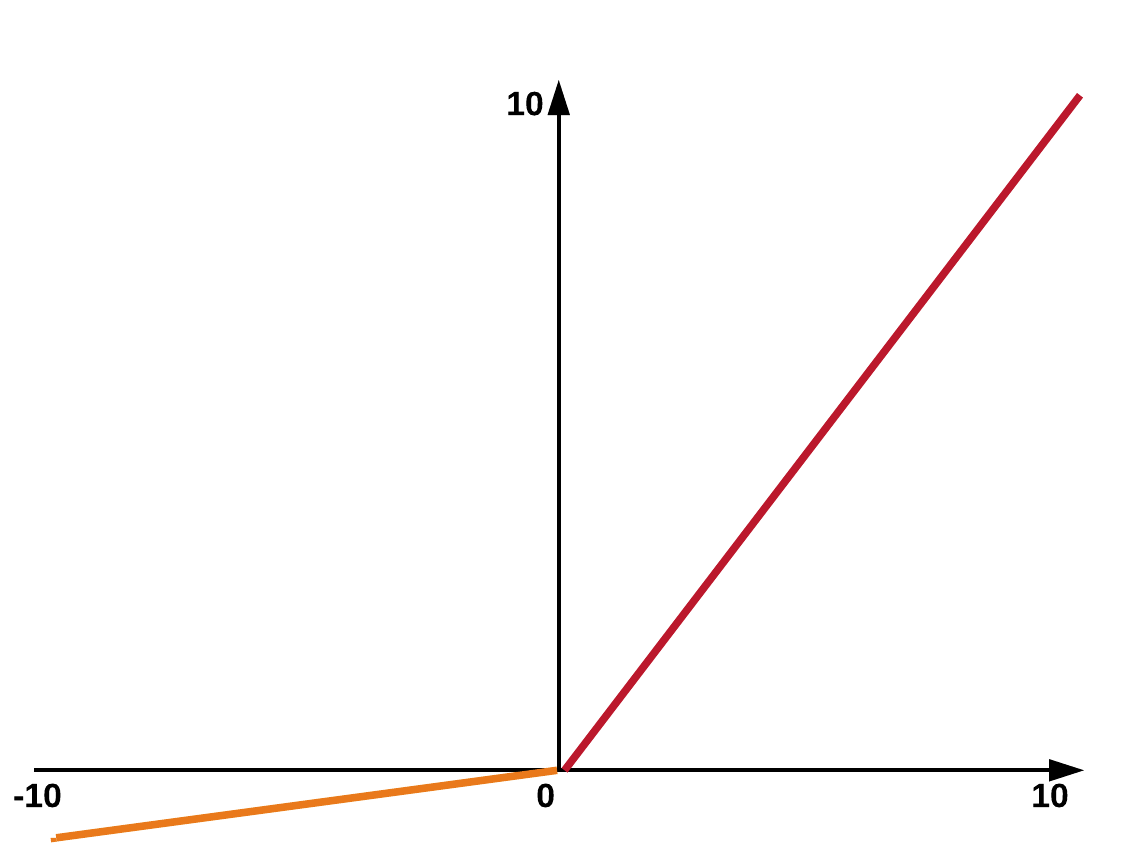
\includegraphics[height=2in]{image/relu}
    \caption{Función Leaky Relu}
    \label{fig:my_label}
\end{figure}

La elección de la función de activación para una capa de una red neuronal depende de los valores de salida que se requieren y de las propiedades de la función de activación utilizada. Por ejemplo, si se trabajan con probabilidades, podría pensarse en usar la función de activación \textbf{Sigmoide} dado que esta función tiene la salida acotada entre 0 y 1, si se trabaja con valores positivos se pensaría en usar la función \textbf{Relu} que anula los valores negativos y para valores generales, se pensaría en usar la función de activación \textbf{Lineal}.

En esquemas con más de una capa, uno preferiría usar la función \textbf{Leaky Relu} en lugar de la \textbf{Relu}, la cual permite ser más permisivo al no anular completamente ciertas neuronas y por el mismo motivo, se prefiere usar la función \textbf{tanh} en lugar de la \textbf{Sigmoide}.




% \section{Ejercicio 2}



% \section{Ejercicio 3}

El ejercicio 3 solicita implementar una red neuronal (sin POO) de dos capas densas para resolver el problema de CIFAR-10. La primera capa tiene cien neuronas y tiene la función de activación sigmoidal. La segunda capa tiene diez neuronas y activación lineal.
Se propone utilizar la función de costo MSE con regularización L2.

En primer lugar se arma el grafo computacional, y luego se programa el algoritmo de \textbf{backpropagation} para resolver el problema.
El grafo que describe este problema es el siguiente:

\begin{figure}[H]
    \centering
    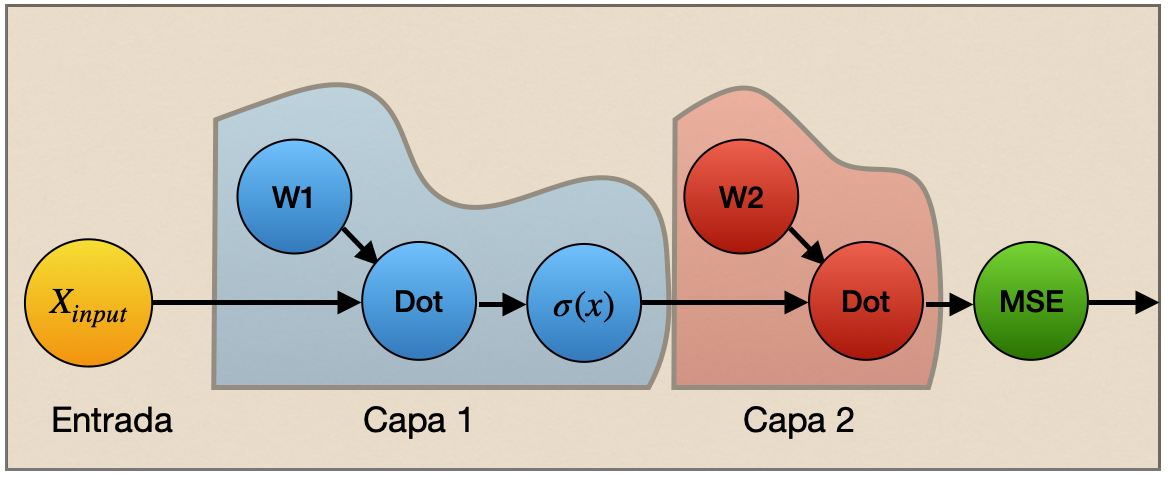
\includegraphics[height=1.5in]{image/graph3}
    \caption{Grafo computacional del problema 3}
    \label{fig:my_label}
\end{figure}

El programa comienza definiendo los hiperparámetros del problema:
\begin{verbatim}
nclases = 10            # salida
nintermedia = 100       # intermedia
batch_size = 256        # Batch size
n_epocas = 100           # Cantidad de épocas
learning_rate = 1e-7    # Learning rate
reg_lambda = 1e-3       # Coeficiente de regularización
n_train_data = 5000     # Cantidad de datos que se usarán para entrenar

\end{verbatim}
A continuación se cargan los datos de cifar y se acomodan las matrices para que puedan ser manipuladas de manera conveniente según se hizo en el Trabajo Práctico 1.
Para contribuir con la estabilidad del código se resta la media de los datos de entrenamiento tanto a los datos de \textbf{testing} como de \textbf{training} y a la diferencia se la divide por la desviación estándar de los datos de training.
Se definen matrices para expresar la salida de la red de manera que cada columna de la matriz de salida representa una clase del conjunto de datos, es decir para CIFAR-10, la cantidad de columnas de la matriz de salida es 10. Entonces, la información de a qué clase pertenece una imagen de CIFAR-10 (información almacenada en el vector \textbf{y}) se escribiría por ejemplo: 0100000000 para representar la clase 2 y 0000000001 para representar la clase 10.

Para el entrenamiento de la red neuronal, se implementó el método de \textit{Backpropagation} utilizando mini batches.
El algoritmo de \textbf{backpropagation} se realizó siguiendo el grafo computacional anteriormente presentado y llamando a las funciones de costo, de activación y gradientes correspondientes.
Además, para el cálculo de la Loss (función de costo) se aplicó la regularización L2. La función Loss se calcula haciendo:
\begin{equation*}
    Loss = \frac{1}{n} f(\hat{y}, y) + reg,
\end{equation*}
donde $n$ es el número de mini batches, $f$ es la función de costo, $\hat{y}$ es el vector de salida estimado, $y$ es el vector de salida esperado y $reg$ es la función de regularización que se calcula como:
\begin{equation*}
    reg = \sum W_1^2 + \sum W_2^2.
\end{equation*}

Realizando el algoritmo de \textit{Backpropagation} y la actualización de los pesos W, se obtienen las siguientes gráficas para el Accuracy y la Loss utilizando la función de costo MSE y con la función sigmoide como función de activación en ambas capas:

\begin{figure}[H]
     \centering
     \begin{subfigure}[b]{0.45\textwidth}
         \centering
         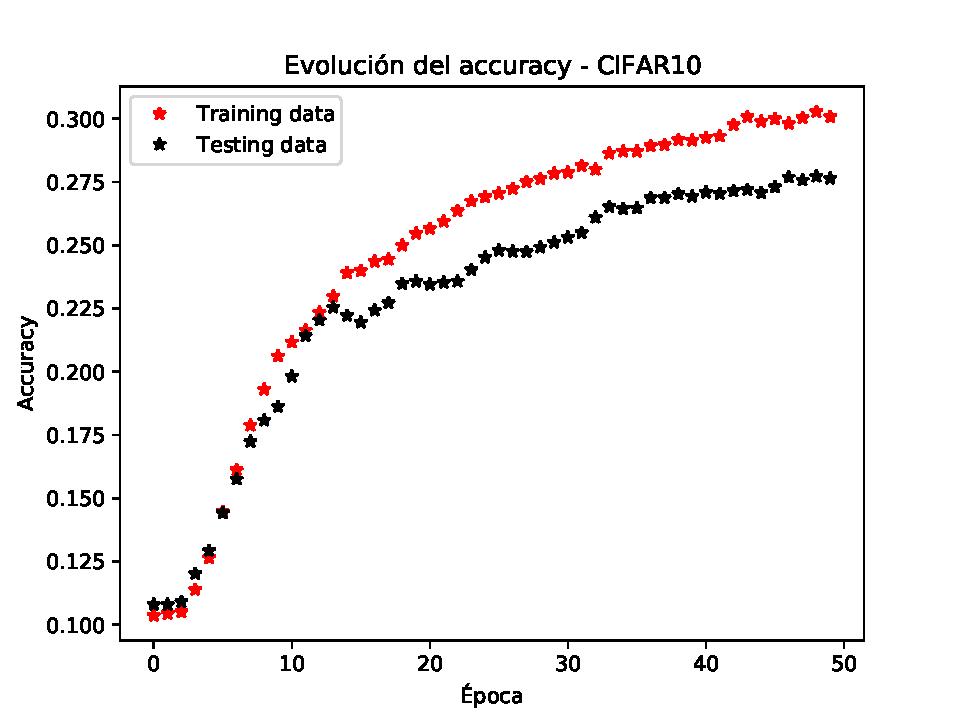
\includegraphics[width=\textwidth]{image/EJ3_Acc_SIG_LIN_MSE.pdf}
         \caption{Accuracy para el problema de CIFAR 10 aplicando Backpropagation}
         \label{fig:acc6a}
     \end{subfigure}
     \hfill
     \begin{subfigure}[b]{0.45\textwidth}
         \centering
         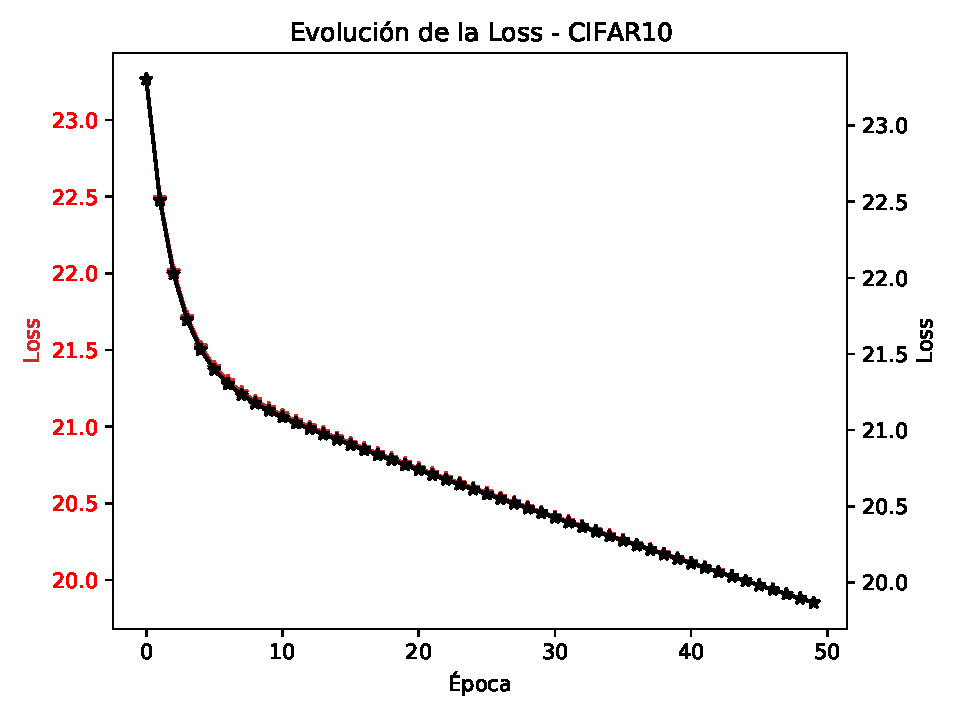
\includegraphics[width=\textwidth]{image/EJ3_Loss_SIG_LIN_MSE.pdf}
         \caption{Loss para el problema de CIFAR 10 aplicando Backpropagation}
         \label{fig:loss6a}
     \end{subfigure}
        % \caption{Resultados para la segunda arquitectura presentada para resolver el problema de la regla XOR con dos capas densas}
        % \label{fig:resu6a}
\end{figure}

Finalmente, se vio cómo cambia el accuracy cuando se utilizan respectivamente los métodos MSE (\textit{Mean Squared Error}), SVM (\textit{Support Vector Machine})y CCE (\textit{Categorical Cross Entropy}) como funciones de costo. En la siguiente figura se muestran los resultados.

\begin{figure}[H]
    \centering
    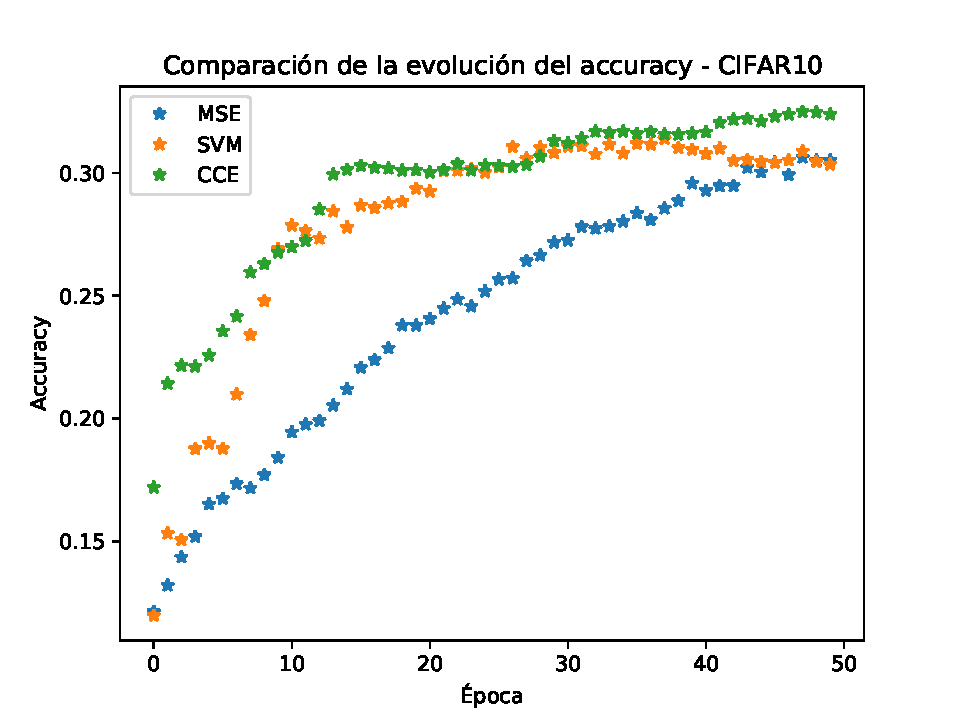
\includegraphics[height=3in]{image/EJ3comparacion2.pdf}
    \caption{Comparación de las accuracy de la red para las funciones de costo MSE, SVM y CCE.}
    \label{fig:ej3}
\end{figure}

De esta figura se ve que el método que alcanza un accuracy más alto es el CCE de SoftMax con un máximo de 38\% para 50 épocas y el método que usa MSE igualó al SVM en las 50 épocas en un valor de 30\%.



% \section{Conclusiones}
Se puede llegar a la conclusión de que se logró alcanzar los objetivos propuestos al principio del trabajo. También, fue posible unificar todos los conocimientos adquiridos a lo largo de la materia, es decir la cinemática directa e inversa de un manipulador robótico, en conjunto con la aplicación de técnicas de \textit{motion planning}. 
Para lograr tal finalidad, se recurrió a la simulación, en la cual fue posible poner a prueba los estudios teóricos realizados sobre el RM-501, verificando que las matrices obtenidas eran las correctas, y que en conjunto con la técnica aplicada para el reconocimiento de imagen, el robot fue capaz de reconocer entre distintas piezas, buscárlas, tomárlas, y depositarlas en una ubicación final deseada. Además, con el algoritmo de Dijkstra implementado sobre tres dimensiones, el robot pudo esquivar distintos obstáculos para cumplir su objetivo sin colisionar con los mismos.

Se puede concluir, que se lograron alcanzar los objetivos de la materia, adquiriendo conocimientos sobre el funcionamiento mecánico de los manipuladores robóticos, y además aprender más aún sobre el lenguaje de programación \textit{Python 3}, en especial de los paquetes \textit{OpenCV} para tratamiento de imágenes, \textit{NumPy} para el tratamiento de matrices y funciones matemáticas de alto nivel y \textit{Panda3D} para la creación de entornos y movimientos tridimensionales.


% \section{Conclusiones}
Se puede llegar a la conclusión de que se logró alcanzar los objetivos propuestos al principio del trabajo. También, fue posible unificar todos los conocimientos adquiridos a lo largo de la materia, es decir la cinemática directa e inversa de un manipulador robótico, en conjunto con la aplicación de técnicas de \textit{motion planning}. 
Para lograr tal finalidad, se recurrió a la simulación, en la cual fue posible poner a prueba los estudios teóricos realizados sobre el RM-501, verificando que las matrices obtenidas eran las correctas, y que en conjunto con la técnica aplicada para el reconocimiento de imagen, el robot fue capaz de reconocer entre distintas piezas, buscárlas, tomárlas, y depositarlas en una ubicación final deseada. Además, con el algoritmo de Dijkstra implementado sobre tres dimensiones, el robot pudo esquivar distintos obstáculos para cumplir su objetivo sin colisionar con los mismos.

Se puede concluir, que se lograron alcanzar los objetivos de la materia, adquiriendo conocimientos sobre el funcionamiento mecánico de los manipuladores robóticos, y además aprender más aún sobre el lenguaje de programación \textit{Python 3}, en especial de los paquetes \textit{OpenCV} para tratamiento de imágenes, \textit{NumPy} para el tratamiento de matrices y funciones matemáticas de alto nivel y \textit{Panda3D} para la creación de entornos y movimientos tridimensionales.


\begin{thebibliography}{9}
\bibitem{regresion}
Julien Jacques, Linear Regression in High Dimension and/or for Correlated Inputs. Article in EAS Publications Series · January 2015. \url{https://www.researchgate.net/publication/276249836}
\bibitem{ariel} 
Ariel Curiale, German Matos, \textit{Notas de la cátedra: Aprendizaje Profundo y Redes Neuronales Artificiales}.
\url{https://classroom.google.com/u/2/c/MTQxNDcxMTM5NjEx}
\bibitem{stanford} 
Fei-Fei Li, \textit{Convolutional Neural Networks for Visual Recognition}.
\url{http://cs231n.stanford.edu/2017/}

\bibitem{tomas}

Códigos del TP1: \url{https://github.com/TomasLiendro/Deep_Learning/blob/master/TP1_Introduction\%20to\%20ML/}
\end{thebibliography}
% \end{document}

% 
\begin{thebibliography}{9}
\bibitem{regresion}
Julien Jacques, Linear Regression in High Dimension and/or for Correlated Inputs. Article in EAS Publications Series · January 2015. \url{https://www.researchgate.net/publication/276249836}
\bibitem{ariel} 
Ariel Curiale, German Matos, \textit{Notas de la cátedra: Aprendizaje Profundo y Redes Neuronales Artificiales}.
\url{https://classroom.google.com/u/2/c/MTQxNDcxMTM5NjEx}
\bibitem{stanford} 
Fei-Fei Li, \textit{Convolutional Neural Networks for Visual Recognition}.
\url{http://cs231n.stanford.edu/2017/}

\bibitem{tomas}

Códigos del TP1: \url{https://github.com/TomasLiendro/Deep_Learning/blob/master/TP1_Introduction\%20to\%20ML/}
\end{thebibliography}
% \end{document}
% \input{problema}
% \newpage
% \input{estudiodemercado}
% \newpage
% \input{estudiotecnico}
\end{document} 
